\documentclass[12pt,a4paper,fontset=none]{ctexart}
\usepackage{ctex}
\usepackage{emptypage} 
\usepackage{fancyhdr}
\usepackage{amsmath,amsfonts,amssymb,mathtools}
\usepackage{graphicx}%插入图片用的宏包
\usepackage{mathptmx}
\usepackage{booktabs}
\usepackage[labelfont=bf]{caption}
\usepackage{indentfirst}
\usepackage{caption}
\usepackage{enumitem}
\usepackage[marginal]{footmisc}
\usepackage{subfigure}
\usepackage{fontspec}
\usepackage{geometry}
\usepackage{setspace}
\usepackage{listings}
\usepackage{xcolor}
\usepackage{float}
\usepackage{forest}
\usepackage{algorithm,algpseudocode,float}%算法基础宏包
\usepackage{algorithmicx}%算法基础宏包,注意小写
\usepackage{algpseudocode}%算法拓展宏包,函数,Return
\usepackage{lipsum}
\newgeometry{left=3cm,top=2.5cm,bottom=2.5cm,right=3cm}
\setmainfont{Times New Roman}
\setCJKmainfont[BoldFont=SimHei,ItalicFont=KaiTi]{SimSun}
\lstset{
	backgroundcolor=\color{green!10!blue!15},
	rulesepcolor= \color{red!40!blue!100},
	breaklines=true,
	breakatwhitespace=false,
	numbers=left, 
	numberstyle= \small,
	keywordstyle= \color{blue},
	commentstyle=\color{gray}, 
	frame=shadowbox
}
\forestset{ 
  default preamble={ 
    font=\large, 
    for tree={circle,draw,minimum size = 10mm} 
  } 
}
\CTEXsetup[format={\bfseries}]{section}
\renewcommand{\baselinestretch}{1.5}

\title{\textbf{数据结构与算法第四次作业}}

\author{
\\
\Large{麻超 \quad 201300066}
\\[6pt]
{ \large \textit{南京大学人工智能学院}}\\[2pt]
}

\date{\today}

\begin{document}
\maketitle
\setcounter{page}{1}
\section*{Problem 1}
\subsection*{a}
\begin{center}
	\begin{forest}
		[I[Q[J[H][L[E][M]]][V]][O[T[S][B[R[G][Y]][Z]]][K[C][A[\&[F[P][N[U][D]]][W]][X]]]]]
	\end{forest}
\end{center}
\subsection*{b}
\textbf{解:}前序遍历的结构是[根节点,左子树,右子树],后序遍历的结构是[左子树,右子树,根节点].每一个子树又可以划分为一个完整的[根节点,左子树,右子树]的结构.因此可以考虑用递归的方法解决问题.

首先,preorder的第一个元素和postorder的最后一个元素必然是整个树的根节点.接下来preorder的第二个元素必然是其左子树的根节点,在postorder里面找到它(如在(a)中的元素'Q'),postorder在Q之前的元素即是该二叉树的左子树中的元素,postorder中其他的元素就是该二叉树右子树中的元素.接下来用同样的方法对preorder中左子树和右子树分别作为一个完整的树进行递归即可.

伪代码如下:
\begin{algorithm}
	\renewcommand{\algorithmicensure}{\textbf{Output:}}
	\renewcommand{\algorithmicrequire}{\textbf{Input:}}
	\caption{Construct the tree}
	\label{alg1}
	\begin{algorithmic}
		\Require $pre[],post[]$
		\Function {Construct}{$pre[],post[]$}
		\If{pre.length=0}
		\Return $null$
		\EndIf
		\State $root\gets pre[0]$
		\If {pre.length=1}
		\Return $root$
		\EndIf
		\State L$\gets$ i+1 and post[i]=pre[1]
		\State $root.left\gets Construct(pre[1,L+1],post[0,L])$
		\State $root.right\gets Construct(pre[L+1,N],post[L,N-1])$
		\Return $root$
		\EndFunction
	\end{algorithmic}
\end{algorithm}
假设一共有n个节点,则其时间复杂度为$O(n^2)$.
\subsection*{c}
如果该树为非满二叉树,则无法确定其值.假设有如下tree:

这两个树的前序遍历都是[1,2,3,4],后序遍历都是[3,4,2,1],但这两个树不同,故如果一个树为非满二叉树,无法通过前序遍历和后序遍历构建这个树.
\section*{Problem 2}
\textbf{解:}按照中序遍历的顺序,从这个树的根结点开始右旋,直至左子树为空,然后对右子树进行上述操作,直至二叉树变成升序排列的链.而每进行一次上述的右旋操作,都会将一个不在这样的链上的结点旋转到这样的链上,所以该操作的步数为$O(n)$.

每一棵含n个结点的二叉搜索树都能通过这样的O(n)的步数旋转成右侧伸展的链,接下来将这个链伸展成为一个平衡二叉树即可.当然,由于树的左旋和右旋互为逆操作,在用旋转操作将一个树变为链的时候,必然可以同样地从一个链变为一个树.由于平衡二叉树也是二叉搜索树的一种,所以它也满足同样的性质.

故总共需要$O(n)+O(n)=O(n)$次旋转操作即可以完成这个算法.
\section*{Problem 3}
对于任意一个二叉搜索树,由第二题中的结论,可以知道将其转化为一条链.在这之后,从这条链的底部节点A开始,将A与其父节点进行比较,若A大于父节点,则对A进行左旋,否则对A的子树进行swap操作后左旋,再对B的子树进行swap操作.不断将A与其父节点进行比较可以获得一个根节点为A,A的左子树中所有节点都小于A,右子树的所有节点都大于A的树.且A的左右子节点分别都是向右延展的链,再次对两个子树进行递归即可得到二叉搜索树.

\begin{algorithm}
	\renewcommand{\algorithmicensure}{\textbf{Output:}}
	\renewcommand{\algorithmicrequire}{\textbf{Input:}}
	\caption{Build binary search tree}
	\label{alg2}
	\begin{algorithmic}
		\Require$T$
		\Function{Build}{T.root}
		\State Turn to a chain(T)
		\If {T.length=1 or T.root=null}
		\Return
		\Else
		\State $A=T.bottom()$
		\While {$A.parent\neq null$}
		\If {A.parent<A}
		\State $Left_Rotation(A)$
		\Else
		\State $swap(A)$
		\State 	$Left_Rotation(A)$
		\State $swap(A)$
		\EndIf
		\EndWhile
		\State Build(A->left)
		\State Build(A->right)
		\EndIf
		\EndFunction
	\end{algorithmic}
\end{algorithm}
时间复杂度分析:将一个树转化为链的过程需要进行O(n)次旋转,在计算过程中需要将底部元素与链中其他所有元素进行比较,以及swap操作,总共需要$O(n^2)$次操作.故总的时间复杂度为$O(n^2)$.
\section*{Problem 4}
\begin{figure}[H]
	\centering
	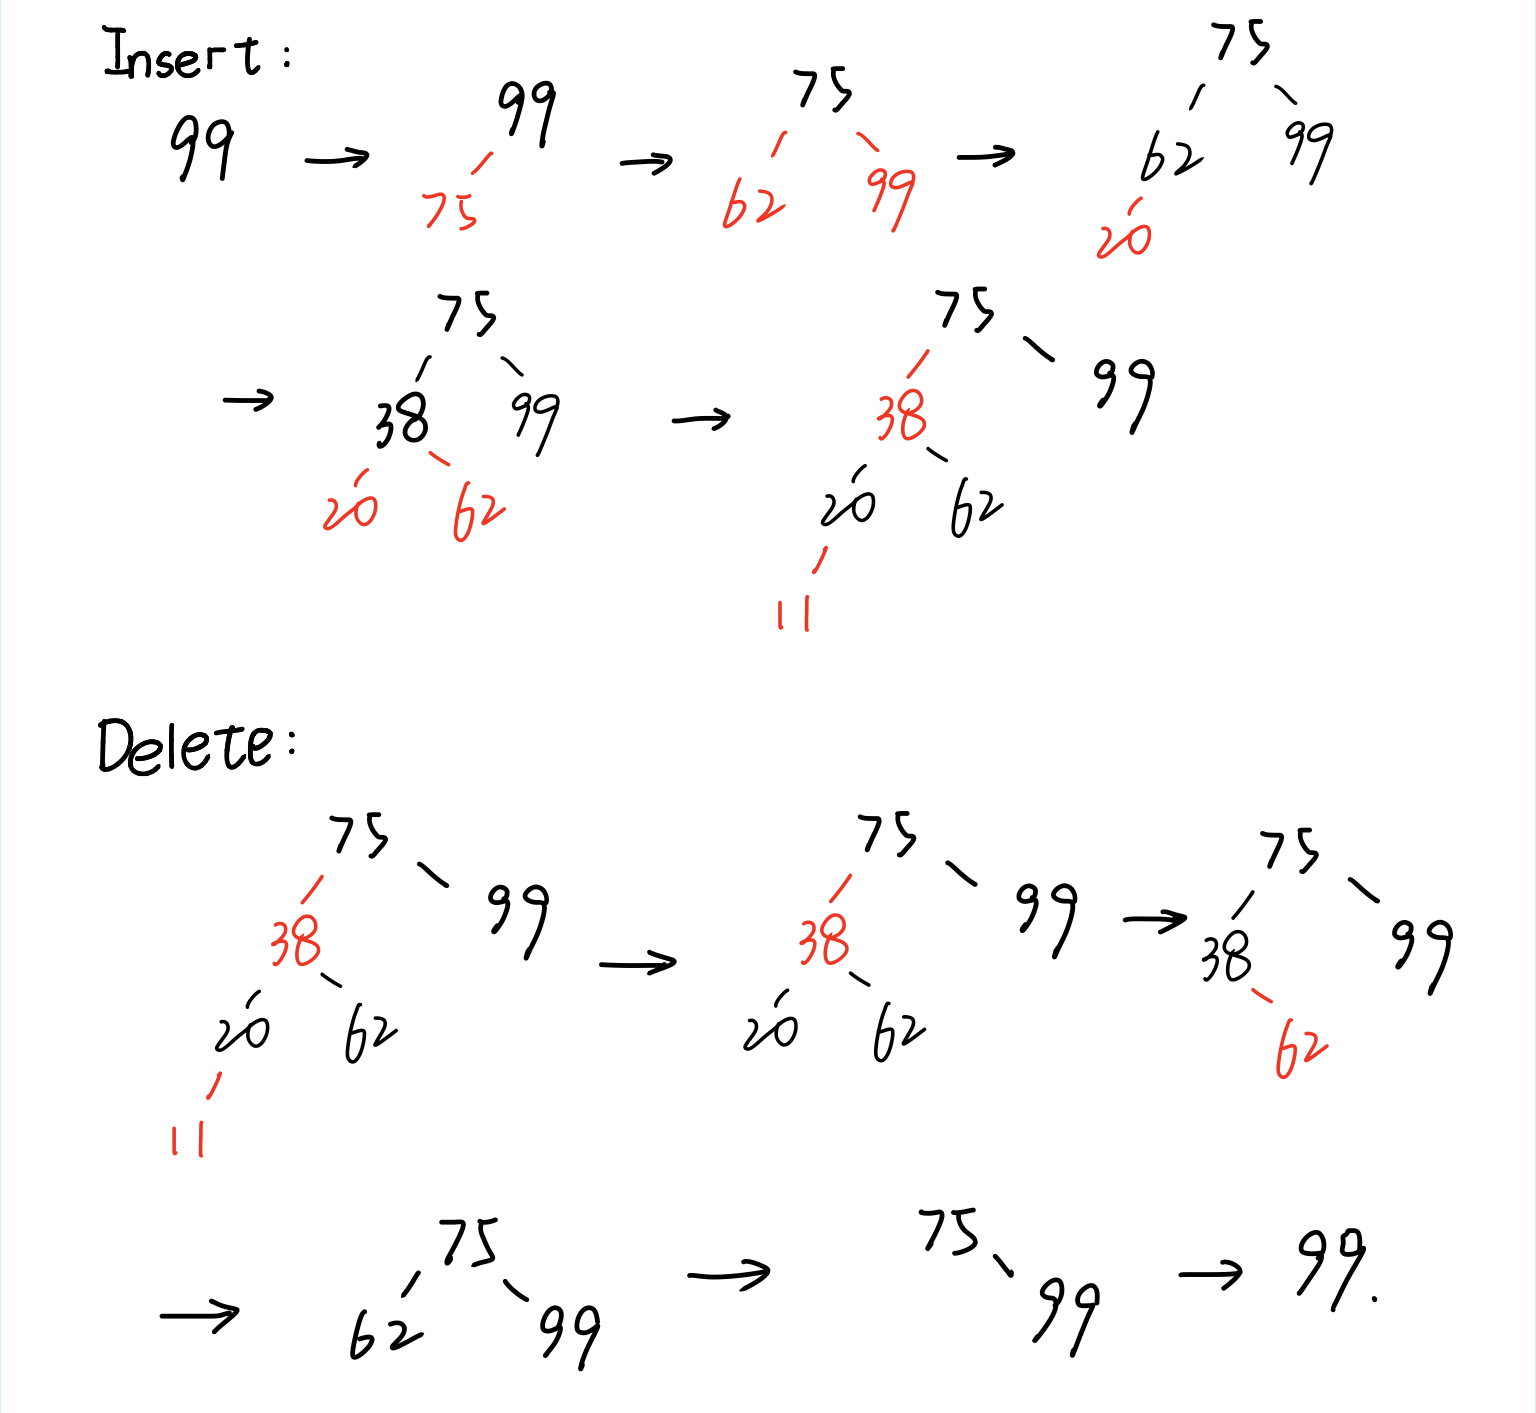
\includegraphics[width=0.7\linewidth]{4题图.png}
\end{figure}
\section*{Problem 5}
\subsection*{a}
假设有一个高度为h的树,则这个树所包含的最小的节点数,设为T(h).则对于这棵AVL树而言,其左右子树中必然至少有一个子树的最大高度等于h-1.由于AVL树的性质(高度平衡),则另一棵AVL树的高度至少为h-2.由于此时T(h)表示的是最小节点数,所以当左右子树都最小时,可以表示T(h),再加上根节点的1,可以知道T(h)=T(h-1)+T(h-2)+1.易得当树的高度为0时,最小结点数为0(空树),当树的高度为1时,最小结点数为1(只有根结点),即T(0)=0,T(1)=1.

由等式(3.25)可得$T(h)=\bigg\lfloor \frac{\phi ^h}{\sqrt{5}}+\frac{1}{2}\bigg\rfloor \leq n$

解得$h\leq \frac{\lg (\sqrt{5})+\lg (n+\frac{1}{2} )}{\lg \phi}\in O(\lg n) $

故有n个节点的AVL tree有O(lg n)的高度.
\subsection*{b}
将一个元素首先按二叉搜索树的顺序添加到AVL树中时,其可能会导致该树高度的变化,导致其不再平衡.通过树的左旋和右旋操作,可以修正由于插入元素导致的平衡性被破坏.

当平衡性被破坏时分为以下四种情况:
\begin{itemize}
	\item 插入到了左子树的左边,可以通过一次右旋操作修正
	\item 插入到了左子树的右边,可以通过先对左子树左旋转化为第一种情况再右旋修正
	\item 插入到了右子树的右边,可以通过一次左旋操作修正
	\item 插入到了右子树的左边,可以通过先对左子树右旋转化为第三种情况再左旋修正
\end{itemize}
\begin{figure}[H]
	\centering
	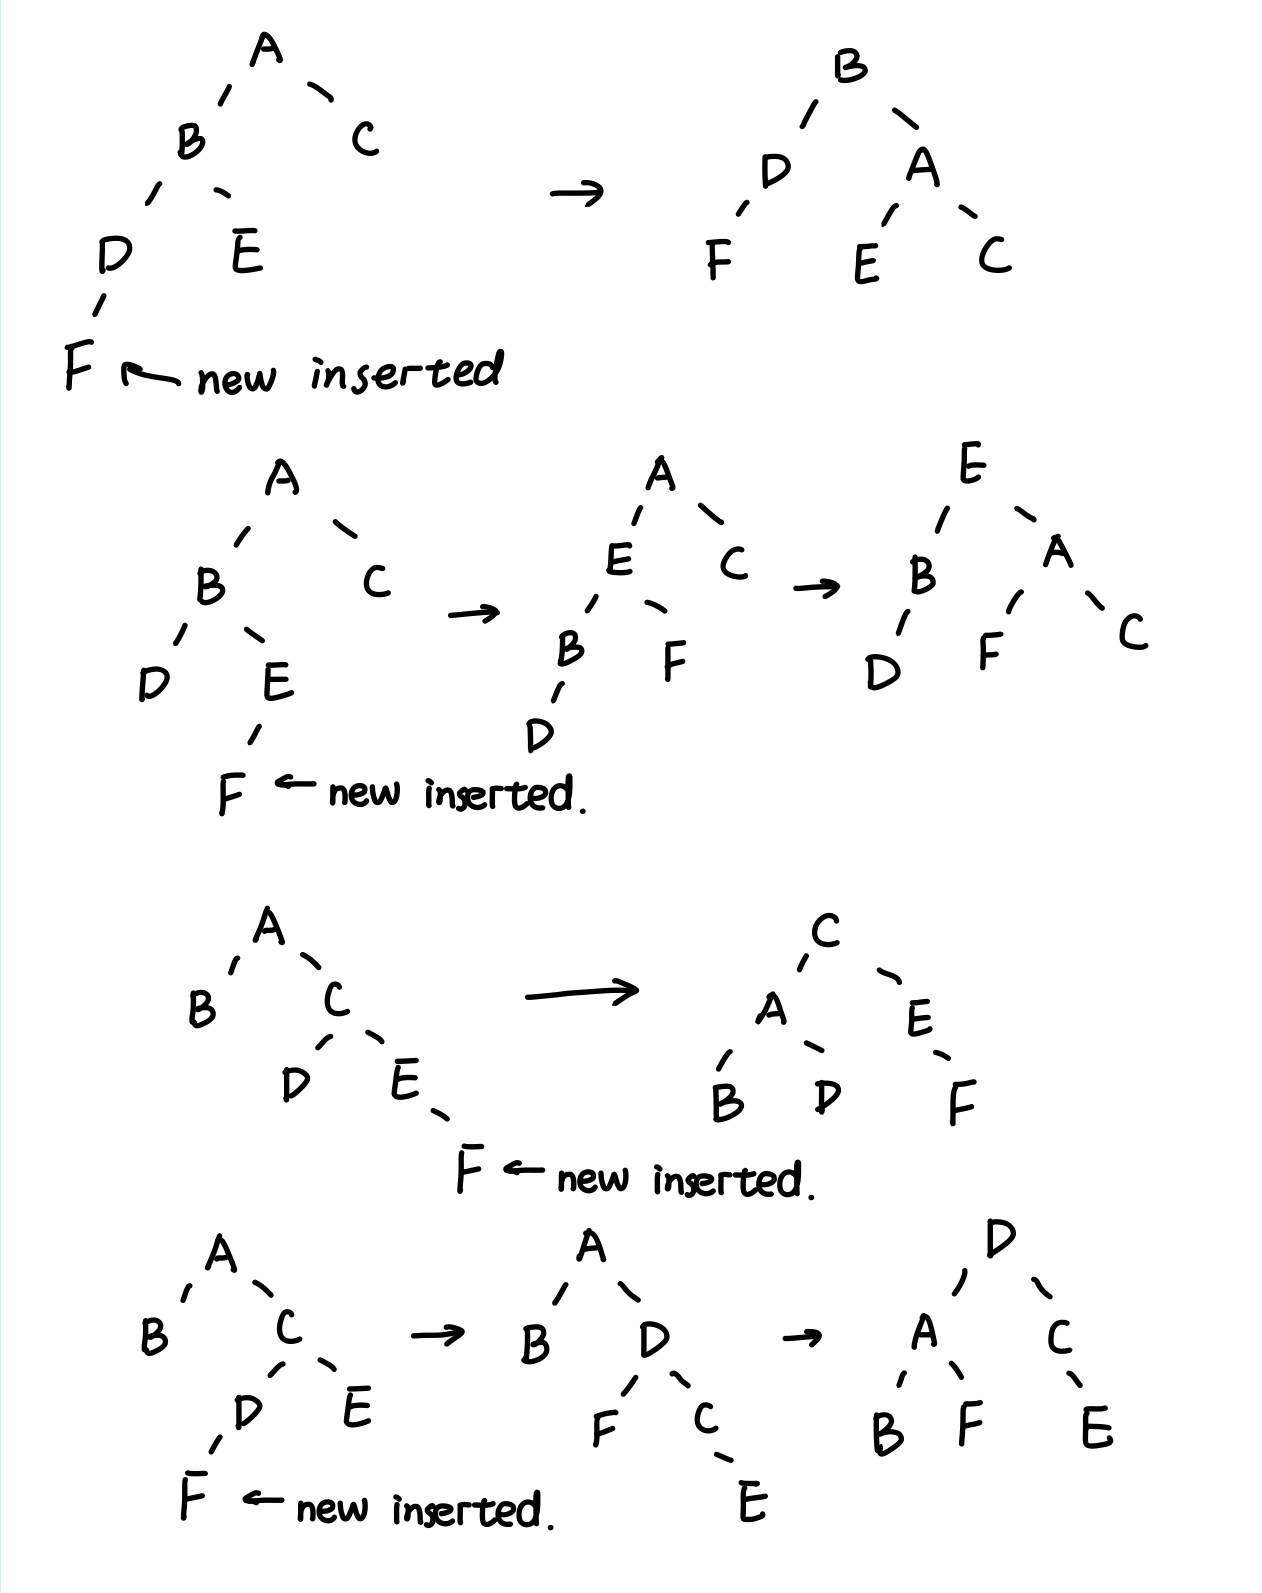
\includegraphics[width=0.7\linewidth]{5题图.png}
\end{figure}
伪代码如下:
\begin{algorithm}
	\renewcommand{\algorithmicensure}{\textbf{Output:}}
	\renewcommand{\algorithmicrequire}{\textbf{Input:}}
	\caption{Balance(x)}
	\label{alg4}
	\begin{algorithmic}
		\Require $tree A,x$
		\Function {Balance}{$A.root,x$}
		\If{$root.key<x$}
		\If{$lefttree.height-righttree.height=2$}\Comment{AVL tree is not balance}
		\If{$root->left.key>x$}\Comment{Condition 1}
		\State $Right-Rotation(root)$
		\Else \Comment{Condition 2}\State $Left-Rotation(root->left)$
		\State $Right-Rotation(root)$
		\EndIf
		\EndIf
		\Else \Comment{插入到右子树}
		\If{$righttree.height-lefttree.height=2$}\Comment{AVL tree is not balance}
		\If{$root->right.key<x$}\Comment{Condition 3}
		\State $Left-Rotation(root)$
		\Else \Comment{Condition 4}\State $Right-Rotation(root->right)$
		\State $Letf-Rotation(root)$
		\EndIf
		\EndIf
		\EndIf
		\EndFunction
	\end{algorithmic}
\end{algorithm}

\subsection*{c}
首先以和二叉搜索树相同的方式将元素插入到AVL tree中,从根节点开始逐次递归地比较每个节点和z的大小关系(如果z大于该节点的值,则应当插入到该节点的右子树中,否则为左子树),直到到达叶节点.最后,从被插入的该节点开始依次递归地向上检查看是否插入操作使得某个子树违背了height-balance的性质,如果违背的话,就通过左旋及右旋操作修正这个错误.直到根节点为止,这样可以首先保证其满足二叉搜索树的性质,其次在旋转过程中,一方面可以保证其height-balance的性质,另一方面也不会改变二叉搜索树的性质.
\begin{algorithm}
	\renewcommand{\algorithmicensure}{\textbf{Output:}}
	\renewcommand{\algorithmicrequire}{\textbf{Input:}}
	\caption{Insert(x,z) }
	\label{alg3}
	\begin{algorithmic}
		\Require $tree A.root\text{ }x,z$
		\If {x=null}
		\State $z.h=0$
		\Return
		\EndIf
		\If {$z.key>x.key$}
		\State $Insert(x->right,z)$
		\If {$x->right=null$}
		\State $x->right=z$
		\EndIf
		\Else
		\State $Insert(x->left,z)$
		\If {$x->left=null$}
		\State $x->left=z$
		\EndIf
		\EndIf
		\State $left-height=-1,right-height=-1$
		\If {$x->left\neq null$}
		\State $left-height=x->left.h$
		\EndIf
		\If {$x->right\neq null$}
		\State $right-height=x->right.h$
		\EndIf
		\State $x.h\gets max(left-height,right-height)+1$
		\State $Balance(x)$
	\end{algorithmic}
\end{algorithm}
\subsection*{d}
在算法中,出现了两次循环,易知这两次循环都只发生了$O(h)=O(\lg n)$次迭代,故运行时间为$O(\lg n)$.在第二个循环,即递归向上检查是否满足AVL的性质时,只需要发生一次旋转,在发生这次旋转之后,该子树的高度将会降低,则对于总的所有元素来说,该树必然已经满足了高度平衡的性质(因为插入过程中只插入了一个元素,最多只会将树的高度增加1),即需要做$O(1)$次旋转.
\section*{Problem 6}
\subsection*{a}
meld操作的基本目标是取两个堆Q1和Q2,并合并它们,结果返回单个堆节点。这个堆节点是包含来自以Q1和Q2为根的两个子树的所有元素的堆的根节点。

如果任一堆为空,则合并将使用空集进行,并且该方法仅返回非空堆的根节点。如果Q1和Q2都不为零,检查是否有Q1>Q2。如果是,交换两者。因此确保Q1<Q2并且合并堆的根节点将包含Q1。然后递归地将Q2与Q1.left或Q1.right合并。在每一次合并时,都会降低一个树的高度,直至某个树为空.

调用meld(Q1,Q2)的期望次数为$\lg x+\lg y\leq 2\lg n$

故期望时间为$O(\lg n)$

\subsection*{b}
FindMin()操作只需要返回该queue的根节点.需要O(1)时间.

DeleteMin()操作只需合并根节点的左右子树,因为最小节点为根节点.

Insert(Q,x)操作首先创建一个只含有x的节点a,然后合并Q和a.

DecreaseKey(Q,x,y):对x的节点的值修改为y,将原节点的父节点指向该节点的指针变为null,显然需要O(1)步操作.然后将Q(new)与该节点再次合并即可.

Delete(Q,x)操作将x的父节点指向x的指针指向x.left,并设置x.left的父节点为x的父节点.然后合并Q(new)与x.right
\end{document}